\documentclass[English, 11pt, twoside, authoryear]{article}
\setlength{\columnsep}{20pt} % column separation width
%\usepackage{txfonts} %font package that is more up to dater than times
\usepackage{natbib}
\usepackage{graphicx}
%\usepackage{wrapfig}
\usepackage{subfigure} %% make it possible to include more than one captioned figure/table in a single float
\usepackage[dvipsnames]{xcolor}
%\usepackage{multicol}
\usepackage{multirow}
%\usepackage{booktabs}
\usepackage{topcapt} % top caption for tables
%\usepackage{a4wide} % makes the text on a page wider
\usepackage{booktabs} % for much better looking tables
\usepackage{paralist} % very flexible & customisable lists (eg. enumerate/itemize, etc.)
\usepackage{verbatim} % adds environment for commenting out blocks of text (\begin{comment} ... \end{comment}) & for better verbatim

%% ---- package for formatting code with line numbers
\usepackage{listings}
\lstset{
backgroundcolor = \color{lightgray},
frame = single, % single,false
framerule = 1.0pt,
rulesep = 0pt,
rulecolor = \color{lightgray},
breaklines = true,
firstnumber = 1,
numbers = left,
numbers = none,
language = Bash,
basicstyle = \ttfamily\small,
showstringspaces = false
}

\usepackage{hyperref}
\hypersetup{%
colorlinks=true,% 
%citecolor=Plum,% 
%linkcolor=green,
%urlcolor=blue% 
}



%
%%%% PAGE DIMENSIONS
\usepackage[margin=2cm, a4paper]{geometry} % for example, change the margins to 2 inches all round
%%\geometry{landscape} % set up the page for landscape
%% read geometry.pdf for detailed page layout information
\usepackage{lscape} % offers landscape environment, \begin{landscape}
%
%%%% HEADERS & FOOTERS
\usepackage{fancyhdr} % This should be set AFTER setting up the page geometry
\pagestyle{fancy} % options: empty , plain , fancy
%%\renewcommand{\headrulewidth}{0pt} % customise the layout...
\lhead{Claudius Kerth} % alined left in header
\chead{\textbf{Kaleidoscope Utils Documentation}}  % alined centrically in header
\rhead{\today}  % alined right in header
\usepackage{lastpage} % in order to call the number of the last page in the footer
\lfoot{}
\cfoot{}
\rfoot{\thepage ~of \pageref{LastPage}}
%
%%%% SECTION TITLE APPEARANCE
%%\usepackage{sectsty}
%%\allsectionsfont{\sffamily\mdseries\upshape} % (See the fntguide.pdf for font help)
%% (This matches ConTeXt defaults)
%
%%%% ToC APPEARANCE
%%\usepackage[nottoc,notlof,notlot]{tocbibind} % Put the bibliography in the Table of Contents
%%\usepackage[titles]{tocloft} % Alter the style of the Table of Contents
%%\renewcommand{\cftsecfont}{\rmfamily\mdseries\upshape}
%%\renewcommand{\cftsecpagefont}{\rmfamily\mdseries\upshape} % No bold!
%
%
\begin{document}
%%%%% TITLE
%
\title{ Documentation for \textsf{Kaleidoscope Utils}  \\
\vspace{20pt}
\normalsize{using \textsf{Kaleidoscope} for bat call identification and analysis, free version 5.1.9g}\vspace{100pt}}

%
%
\author{Claudius Kerth\\Wolfener Str. 18\\04155 Leipzig\\Germany\\email: \texttt{claudiuskerth@gmail.com}}
%%double-shlash for line breaks
%% \texttt sets the letters in monospace font, might be interesting for typesetting DNA sequences
%
%
\date{~} % tilde for no date, \today for current date
%
%
%\thispagestyle{plain}
%
%
%%%% BEGIN DOCUMENT
%
%
\maketitle
%
%%Because the maketitle command has just been used, it automatically
%%issues \thispagestyle{plain} which overrides the fancy headings for
%%this page.  Must now tell Latex to override this!

\thispagestyle{empty} % remove page number from title page
%
%
\tableofcontents % uncomment to insert the table of contents
%
%
\clearpage % inserts pagebreak, I think
\setcounter{page}{1} % reset page counter, don't want to count the title page
%
% Requires the booktabs if the memoir class is not being used
%
%
%%\setlength{\columnsep}{20pt} % sets the distance between the text columns
%%\begin{multicols*}{2} % multicol package needs to be installed for this, sets the number of text columns per page to two
%
%
%%%%%%%%%%%%%%%%%%%%%%%%%%%%%%%%%%%%%%%
\onecolumn


%
%
%
\section{Pre-processing \texttt{meta.csv}}

%
%
%
\subsection{How to make MANUAL ID column in \texttt{meta.csv} blank}
%
%
%
After batch processing, the MANUAL ID column in \texttt{meta.csv} contains the same as the AUTO ID column. This is unfortunate, since it is not clear whether a manual review of the auto id has taken place. An empty MANUAL ID field should mean that for this recording no manual inspection has been done yet. One way to make this column blank before manual inspection would be to open \texttt{meta.csv} in a spreadsheet and clearing the column manually. Another possibility is to use the following command line (one line):

\begin{lstlisting}
perl -F"," -i -lane 'if($.==1){print; for($i=0;$i<@F;$i++)
{if($F[$i] =~ /^MANUAL ID$/){$Spalte=$i}}}
else{$F[$Spalte] = ""; print join(",", @F)}' meta.csv
\end{lstlisting}

This command could be part of a pre-processing script for \texttt{meta.csv}.

%
%
%
\subsection{How to sort \texttt{meta.csv} by date and time}
%
%
%
Under \fbox{Kaleidscope Help} $\rightarrow$ \fbox{Metadata Panel} $\rightarrow$ \fbox{Results Window} on can find:

\begin{quote}
Rows can be sorted by clicking on column headers. Clicking on a column header again will reverse the sort order. Sort by multiple columns. For example, click on one column header to sort the data in that column, then click on a second column header to sort the second column. In this case, all the matching second column rows will be together and sorted in the order of the first column.
\end{quote}

This works sort of after pressing 10 times and checking if the result is really sorted according to the two columns DATE and TIME. I generally would like to work chronologically through a recording session from earliest to last. The following command (one line) can sort \texttt{meta.csv} first by date then by time:

\begin{lstlisting}
cat <(head -1 meta.csv) <(tail +2 meta.csv | sort -t, -k5 -k6) 
> meta_sorted.csv
\end{lstlisting}

%
%
%
\subsection{How to add a line number column to meta.csv}
%
%
%
Occasionally I want to sort the table in the Results window (\texttt{meta.csv}) of \textsf{K} Viewer according to AUTO ID or maybe some other column. In order to quickly restore the previous chronological sorting order it would be nice to have an extra column with line numbers (or \underline{n}umber of \underline{r}ecord) assigned after chronological sorting. Again, one could open \texttt{meta.csv} in a spreadsheet to add this column or one could use the following command line:

\begin{lstlisting}
perl -F"," -ne 'chomp; if($.==1){print $_, ",NR", "\n";}
else{print $_, ",", $.-1, "\n";}' meta_sorted.csv 
> meta_sorted_NRcolumn.csv
\end{lstlisting}

Note, that the NR column cannot be added as the first column or \textsf{K} viewer will not be able to open the file.

%
%
%
\subsection{Noise detection}
%
%
%

With the free version of Kaleidoscope, noise detection only works by copying files to the output directory, unfortunately. The \texttt{meta.csv} file does not contain an indication of whether a file got detected as noise. However, in the output of the Pro version of \textsf{K}, one can find in the \texttt{id.csv} file (only produced by the pro version) files that got designated as noise.

%
%
%
\subsubsection{How to add the noise label to \texttt{meta.csv}}
%
%
%
When batch processing with the Kaleidoscope free version one has to copy input files to the output directory. The required settings are shown in figure \ref{Batch_proc_for_noise_detection}. Recordings that are detected as noise are then moved to a subdirectory called NOISE in the output directory.

\begin{figure}[htbp]
\begin{center}
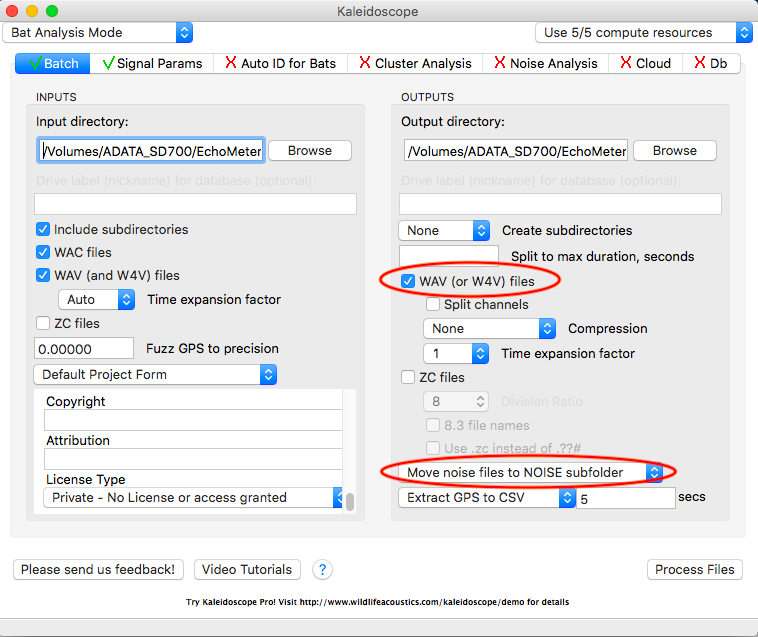
\includegraphics[width=.7\textwidth]{Fig/Batch_proc_for_noise_detection}
\caption{Necessary setting to allow noise detection with the free version of Kaleidoscope.}
\label{Batch_proc_for_noise_detection}
\end{center}
\end{figure}

The following command (one line) inserts the word "Noise" into the AUTO ID column of \texttt{meta.csv} if the recording has been detected as noise:

\begin{lstlisting}
perl -F, -lane 'if($.==1){print}else{
($file = $F[2]) =~ s/^(.*)\.(.*)/$1_000.$2/; 
$file = "NOISE/" . $file; 
if(-e $file){$F[17] = "Noise"}; 
print join(",", @F)
}' meta.csv > meta_with_noise_in_Auto_ID.csv
\end{lstlisting}

Note that on line 2 in the command, the file name taken from \texttt{meta.csv} has to be modified: the string "\_000" has to be inserted. The copied files in the output directory of batch processing have this additional string, but \texttt{meta.csv} contains the names of the source files. The command checks whether a recording file has been put into the subfolder NOISE.

%
%
\subsection{How to add more than one species label per recording file}
%
%

Under \fbox{Kaleidoscope Help} $\rightarrow$ \fbox{Reference Guide} $\rightarrow$ \fbox{Metadata Panel} one can find the following info:

\begin{quote}
To assign multiple manual IDs, hold the Control key down while pressing one of the user-defined buttons (or the corresponding shortcut key). This will add the label to the Manual ID field, separating multiple entries with commas while also disabling the Auto next file button. 
\end{quote}

On a Mac press the \fbox{cmd} key instead of the \fbox{ctrl} key. The choice of a comma to separate species labels is unfortunate since \texttt{meta.csv} is comma separated. I would therefore recommend to edit multi-species labels so that they are separated by a semicolon.

Usually, when you save \texttt{meta.csv} with \textsf{K} it will add double quotes around each field entry, which disrupts further command line manipulation of this important file. If you have multi-species labels that are separated by a comma the use the following command line to separate them by a semicolon:

\begin{lstlisting}[numbers=none]
perl -F/\",\"/  -i -lane 
'map {tr/,/;/} @F; print join(",", @F)' meta.csv
\end{lstlisting}


Afterwards, it is save to remove double quotes:

\begin{lstlisting}[numbers=none]
tr -d '"' < meta.csv > meta_noquotmark.csv
\end{lstlisting}



%
%
%
\subsection{How to add notes}
%
%
%

In the Metadata panel there is a field called notes. Under \fbox{Kaleidoscope Help} $\rightarrow$ \fbox{Reference Guide} $\rightarrow$ \fbox{Metadata Panel} it says:
\begin{quote}
Under Notes there is an \emph{editable} field which contains field notes and GUANO format metadata if present.
\end{quote}
I have tried to edit this field with the free version of \textsf{K}, but it is not saved. It may be that only during batch processing, information that pertains to the whole session of recordings can be saved here. Notes for individual recordings cannot be saved here, at least with the free version of \textsf{K}.

A workaround, although more error prone than editing directly in the results window of \textsf{K} Viewer, is to create an \texttt{id\_notes.csv} file that contains a selection of columns from \texttt{meta.csv} and then open that file in a spreadsheet application for editing together with \textsf{K} Viewer. Since \texttt{meta.csv} already contains a NOTES column, I suggest naming the new notes column "ID NOTES".

The following command will display a numbered list of column headers from \texttt{meta.csv}. 

\begin{lstlisting}[numbers=none]
head -1 meta.csv  | tr ',' '\n' | nl

     1	INDIR
     2	FOLDER
     3	IN FILE
     4	DURATION
     5	DATE
     6	TIME
     7	HOUR
     8	DATE-12
     9	TIME-12
    10	HOUR-12
    11	LATITUDE
    12	LONGITUDE
    13	MODEL
    14	SERIAL NO
    15	FIRMWARE
    16	PREFIX
    17	NOTES
    18	AUTO ID
    19	PULSES
    20	MATCHING
    21	MATCH RATIO
    22	MARGIN
    23	FILES
    24	MANUAL ID
    25	ORGID
    26	USERID
    27	REVIEW ORGID
    28	REVIEW USERID
    29	INPATHMD5
    30	NR
\end{lstlisting}

I can then use the following command to create a copy of \texttt{meta.csv} with a selection of columns
\begin{lstlisting}[numbers=none]
cut -d, -f3,5-6,18,24,30 meta.csv > id_notes.csv
\end{lstlisting}

The new "ID NOTES" column can be added to \texttt{id\_notes.csv} in the spreadsheet application. With it \texttt{id\_notes.csv} will have 7 columns. The file format needs to stay the same.

%
%
\subsection{Preprocessing script}
%
%

The command lines documented above have been wrapped up in a script called \texttt{preprocessing\_meta.sh}. It should be run from within the output directory of \textsf{K} batch processing and before manual review of auto id. The scripts takes no command line arguments.
It produces a new \texttt{meta.csv} while preserving the original in \texttt{meta\_orig.csv}.

Specifically the script does the following:
\begin{enumerate}
\item check for signs that preprocessing has already been run on meta.csv
\item make a backup of the original meta.csv
\item make the MANUAL ID column blank
\item sort \texttt{meta.csv} by date and time
\item add a line number column
\item check if a directory called NOISE exists, if yes, then add noise label to AUTO ID column
\item create \texttt{id\_notes.csv} for note taking in a spreadsheet app
\end{enumerate}


%
%
%
\section{Post-processing \texttt{meta.csv}}
%
%
%

%
%
\subsection{How to remove lines for noise recordings from \texttt{meta.csv}}
%
%

The following command line removes lines from \texttt{meta.csv} that contain the word "noise" (upper or lower case) in the column MANUAL ID:

\begin{lstlisting}
perl -F, -i'.withNoise' -lane'if($.==1)
{print; for($i=0;$i<@F;$i++){if($F[$i] =~ /^MANUAL ID$/){$Spalte=$i}}}
else{print if not $F[$Spalte] =~ /noise/i}' meta.csv
\end{lstlisting}

The command also makes a backup of the \texttt{meta.csv} with lines for noise recordings.

%
%
\subsection{How to join ID NOTES to \texttt{meta.csv}}
%
%

After manual review of recordings in \textsf{K} Viewer, filling the MANUAL ID column and adding corresponding notes to \texttt{id\_notes.csv}, the "ID NOTES" column (here the seventh column) can be joined back to \texttt{meta.csv} with the following command line (one line):

\begin{lstlisting}
join -t, -1 3 -2 1  meta.csv <(cut -d, -f1,7 id_notes.csv) 
> meta_with_id_notes.csv
\end{lstlisting}

The upper command requires that \texttt{id\_notes.csv} is comma-separated and that the id notes made in the spreadsheet contain no commas. The following command line makes sure that the ID NOTES column, which must be the last column of the file, has semicolons instead of commas if they exist:

\begin{lstlisting}[numbers=none]
perl -i -pe'next if not /"$/; ($pre_note, $note) = $_ =~ /(.*,)(".*"$)/; 
$note =~ tr/,/;/; $_ = $pre_note . $note . "\n";' id_notes.csv
\end{lstlisting}

This command should be run before the \textsf{join} command.

%
%
\subsection{How to create a KML file from the \texttt{meta.csv} file after manual id}
%
%

The EMT app creates a KML file for each recording session. It would be nice to create an updated KML file after manual review of the recordings. This is what the programme \texttt{style2kml.pl} does. It takes a \texttt{meta.csv} (usually after reviewing the recordings and filling the MANUAL ID column) as well as a(ny) Session*kml file created by the EMT app and creates a KML that contains Placemarks that show the manual id (not the auto id from the EMT app) and the remaining info in \texttt{meta.csv} in a pop-up table in Google Earth. Note, that the programme relies on the \texttt{ogr2ogr} utility from \href{https://gdal.org/download.html}{GDAL}.

\begin{lstlisting}[language=Perl, backgroundcolor = \color{OliveGreen}, basicstyle=\small\ttfamily\color{white}, keywordstyle=\color{YellowOrange}\bfseries,
identifierstyle=\color{Cyan}\bfseries, stringstyle=\color{BrickRed}, commentstyle=\color{blue}, title=\texttt{style2kml.pl}, numbers=left, numberstyle=\color{black}]
my $usage = "usage: 

$0 --meta <your meta.csv> --EMT_kml <kml from EMT app> [--species <species abbreviation>]

--meta your meta.csv file name (and path)
--EMT_kml any Session*kml file name from EMT app 
[--species species abbreviation as used by Kaleidoscope, e.g. HYPSAV]

prints result to STDOUT
\n";

system("which ogr2ogr > /dev/null") == 0 or die "You need to have the utility ogr2ogr installed and in your PATH.
https://gdal.org/download.html\n";

my ($meta, $EMT_kml, $species);

sub parse_command_line {
    while(@ARGV){
        $_ = shift @ARGV;
        if(/^-{1,2}meta$/){$meta = shift @ARGV;}
        elsif(/^-{1,2}species$/){$species = shift @ARGV;}
        elsif(/^--EMT-kml$/){$EMT_kml = shift @ARGV;}
        elsif(/^-{1,2}h(elp)?$/){die $usage;}
    }
}


parse_command_line();
die $usage unless (defined($meta) && ($meta ne "") && defined($EMT_kml) && ($EMT_kml ne ""));

# extracts the style definition from a session kml produced by EMT app
# we want to reuse the style in our new KML file
sub get_style{
    my $style_fh;
    open($style_fh, "<", $EMT_kml) or die $!; 
    while(<$style_fh>){
        print if /<Style/ .. /<\/Style>/;
    }   
}


# generate KML from the meta.csv file after manual id
my $cmd;
if(defined $species and $species ne ""){
    $cmd = sprintf("ogr2ogr -f KML meta_raw.kml %s -a_srs \'EPSG:4326\' -oo X_POSSIBLE_NAMES=LON\* -oo Y_POSSIBLE_NAMES=LAT\* -oo KEEP_GEOM_COLUMNS=NO -where  \"\\\"MANUAL ID\\\" LIKE \'%%%s%%\'\" ", $meta, $species);
}else{
    $cmd = sprintf("ogr2ogr -f KML meta_raw.kml %s -a_srs \'EPSG:4326\' -oo X_POSSIBLE_NAMES=LON\* -oo Y_POSSIBLE_NAMES=LAT\* -oo KEEP_GEOM_COLUMNS=NO", $meta);
}
system($cmd) == 0 or die $?;


# open the KML to which the style should be added
open (my $metaKML, "meta_raw.kml") or die $!; 
my ($manual_id, $date, $time, @manual_IDs);

# add required style info
# use MANUAL ID for marker style (the Session KML uses AUTO ID)
# add date and time in name tag (for chronological sorting in Google Earth)
while(<$metaKML>){
    print;
    # add the style definition after the Document XML tag
    if(/<Document.*>/){
        print get_style();
        #       print "\n";
    }   
    # add marker style XML tag to each Placemark
    elsif(/"MANUAL ID"/ and /SimpleData/){
        ($manual_id) = $_ =~ />(.*)</;
    }elsif(/<\/ExtendedData>/){
        @manual_IDs = split(/;/, $manual_id);
        # MarkerStyle for first species
        print "\t<styleUrl>#MarkerStyle", $manual_IDs[0], "</styleUrl>\n"; 
        # put manual ids in name tag
        print "\t<name>", join(', ', @manual_IDs), "</name>\n"; 
    }   
}

# clean up
system("rm -f meta_raw.kml") == 0 or die $?;
\end{lstlisting}

%
%
\subsection{Postprocessing script}
%
%

The above commands and programmes are wrapped up in a script called \texttt{postprocessing\_meta.sh}.
It should be run from within the output directory of \textsf{K} batch processing after manual review of auto id's, filling the MANUAL ID column in \texttt{meta.csv} and optionally the ID NOTES column in \texttt{id\_notes.csv}. The script takes the following arguments:
\begin{itemize}
\item a KML file from the EMT app (you can find one in the input directory of \textsf{K} batch processing)
\item a species code to create a KML for a certain species only (optional)
\end{itemize}

Specifically, the script does the following:
\begin{enumerate}
\item make a backup of \texttt{meta.csv} after manual review before post-processing (your work won't get lost!)
\item check that files \texttt{meta.csv} and \texttt{id\_notes.csv} exist
\item remove double quotes and separates multi-species entries in MANUAL ID column by a semicolon instead of comma
\item check if all fields in MANUAL ID column of \texttt{meta.csv} are filled
\item remove carriage returns in \texttt{meta.csv} (created by \textsf{K})
\item add system UID into the column REVIEW USERID of \texttt{meta.csv}
\item add the current date in a new column MANUAL ID DATE of \texttt{meta.csv}
\item replaces commas with semicolons in ID NOTES column of \texttt{id\_notes.csv}
\item join ID NOTES column of \texttt{id\_notes.csv} to \texttt{meta.csv}
\item discard some useless columns from \texttt{meta.csv}
\item discards line with manual id "noise"
\item create a \texttt{meta.kml} file from \texttt{meta.csv} allowing for specification of a \textsf{K} species code to create a KML file for one species only
\end{enumerate}




\end{document}
